\documentclass[10pt,pdf,utf8,russian,aspectratio=169]{beamer}
\usepackage[T2A]{fontenc}
\usepackage[english,russian]{babel}
\usepackage{subfig}
%
% Choose how your presentation looks.
%
% For more themes, color themes and font themes, see:
% http://deic.uab.es/~iblanes/beamer_gallery/index_by_theme.html
%
\mode<presentation>
{
  \usetheme{Boadilla}      % or try Darmstadt, Madrid, Warsaw, ...
  \usecolortheme{seagull} % or try albatross, beaver, crane, ..

  \usefonttheme{structurebold}  % or try serif, structurebold, ...
  \setbeamertemplate{navigation symbols}{}
  \setbeamertemplate{caption}[numbered]
} 


\title[Сложность модели]{Сложность моделей глубокого обучения}
\author{Бахтеев Олег}
\institute{МФТИ}
\date{02.11.2016}

\begin{document}

\begin{frame}
  \titlepage
\end{frame}

% Uncomment these lines for an automatically generated outline.
\begin{frame}{План}
  \tableofcontents
\end{frame}

\section{Сложность модели}
\begin{frame}{Сложность модели}
Мотивация
\end{frame}


\begin{frame}{Принцип минимальной длины описания}
\[
\text{MDL}(\mathbf{f}, \mathbf{X}) = L(\mathbf{f}) + L(\mathbf{X}|\mathbf{f}),
\]
где $\mathbf{f}$ --- модель, $\mathbf{X}$ --- выборка, $L$ --- длина описания в битах.
\\
\[
\text{MDL}(\mathbf{f}, \mathbf{X}) \sim L(\mathbf{f}) + L(\mathbf{W}^*| \mathbf{f}) + L(\mathbf{X}|\mathbf{W}^*, \mathbf{f}),
\]
$\mathbf{w}^*$ --- оптимальные параметры модели.\\


$\mathbf{f}_1: L(\mathbf{f}_1)\qquad L(\mathbf{W}_1^*| \mathbf{f}_1) \qquad \qquad \qquad \qquad \qquad	\qquad L(\mathbf{X}|\mathbf{W}_1^*, \mathbf{f}_1) $\\
$\mathbf{f}_2: L(\mathbf{f}_2)\qquad \qquad L(\mathbf{W}_2^*| \mathbf{f}_2) \qquad \qquad \qquad \qquad L(\mathbf{X}|\mathbf{W}_2^*, \mathbf{f}_2) $\\
$\mathbf{f}_3: L(\mathbf{f}_3)\qquad \qquad \qquad L(\mathbf{W}_3^*| \mathbf{f}_3) \qquad \qquad \qquad \qquad \qquad L(\mathbf{X}|\mathbf{W}_3^*, \mathbf{f}_3) $

\end{frame}

\begin{frame}{MDL и Колмогоровская сложность}
\textbf{Колмогоровская сложность} --- длина минимального кода для выборки на предварительно заданном языке.

\textbf{Теорема об инвариантности кодов}\\
Для двух сводимых по Тьюрингу языков колмогоровской сложность  отличается не более чем на константу, не зависяющую от мощности выборки.\\

Отличия от MDL:
\begin{itemize}
\item Колмогоровская сложность невычислима.
\item Длина кода может зависеть от выбранного языка. Для небольших выборок теорема об инвариантности кодов не дает адекватных результатов.
\end{itemize}
\end{frame}

\begin{frame}{Оптимальная универсальная модель MDL}
Пусть выборка $\mathbf{X}$ лежит в некотором конечном множестве $\mathbb{X}: \mathbf{X} \subset \mathbb{X}$.
%2.20
\[
\text{MDL}(\mathbf{f}, \mathbf{X}) = L(\mathbf{X}|\mathbf{W}^*(\mathbf{X}), \mathbf{f}) + \text{COMP}(\mathbf{f}),
\]
$$ L(\mathbf{X}|\mathbf{W}^*, \mathbf{f}) = -\text{log}p(\mathbf{X}|\mathbf{W}^*(\mathbf{X}), \mathbf{f}), \quad 
\text{COMP} = log \sum_{\mathbf{X}' \in \mathbb{X}} P(\mathbf{X}'|\mathbf{W}^*(\mathbf{X}'), \mathbf{f}).$$

В случае (TODO: уточнить) оценка MDL совпадает с точностью до $o(1)$ с байесовской оценкой правдоподобия (``Evidence''):
\[
	p(\mathbf{X}|\mathbf{f}) = \int_\mathbf{w} p(\mathbf{X}|\mathbf{w})p(\mathbf{w}) d\mathbf{w},
\]
где $p(\mathbf{w})$ --- априорное распределение специанльного вида:
$$
	p(\mathbf{w}) = \frac{\sqrt{|J(\mathbf{w})|}}{\int_{\mathbf{w}'} \sqrt{|J(\mathbf{w'})|}d\mathbf{w'}},
$$
$J(\mathbf{w})$  --- информация Фишера.
\end{frame}	


\begin{frame}{Байесовый подход к сложности}
Правдоподобие модели (``Evidence''):
\[
	p(\mathbf{X}|\mathbf{f}) = \int_\mathbf{w} p(\mathbf{X}|\mathbf{w})p(\mathbf{w}) d\mathbf{w}.
\]


\begin{figure}
  \centering
  \subfloat[Схема выбора модели по правдоподобию]{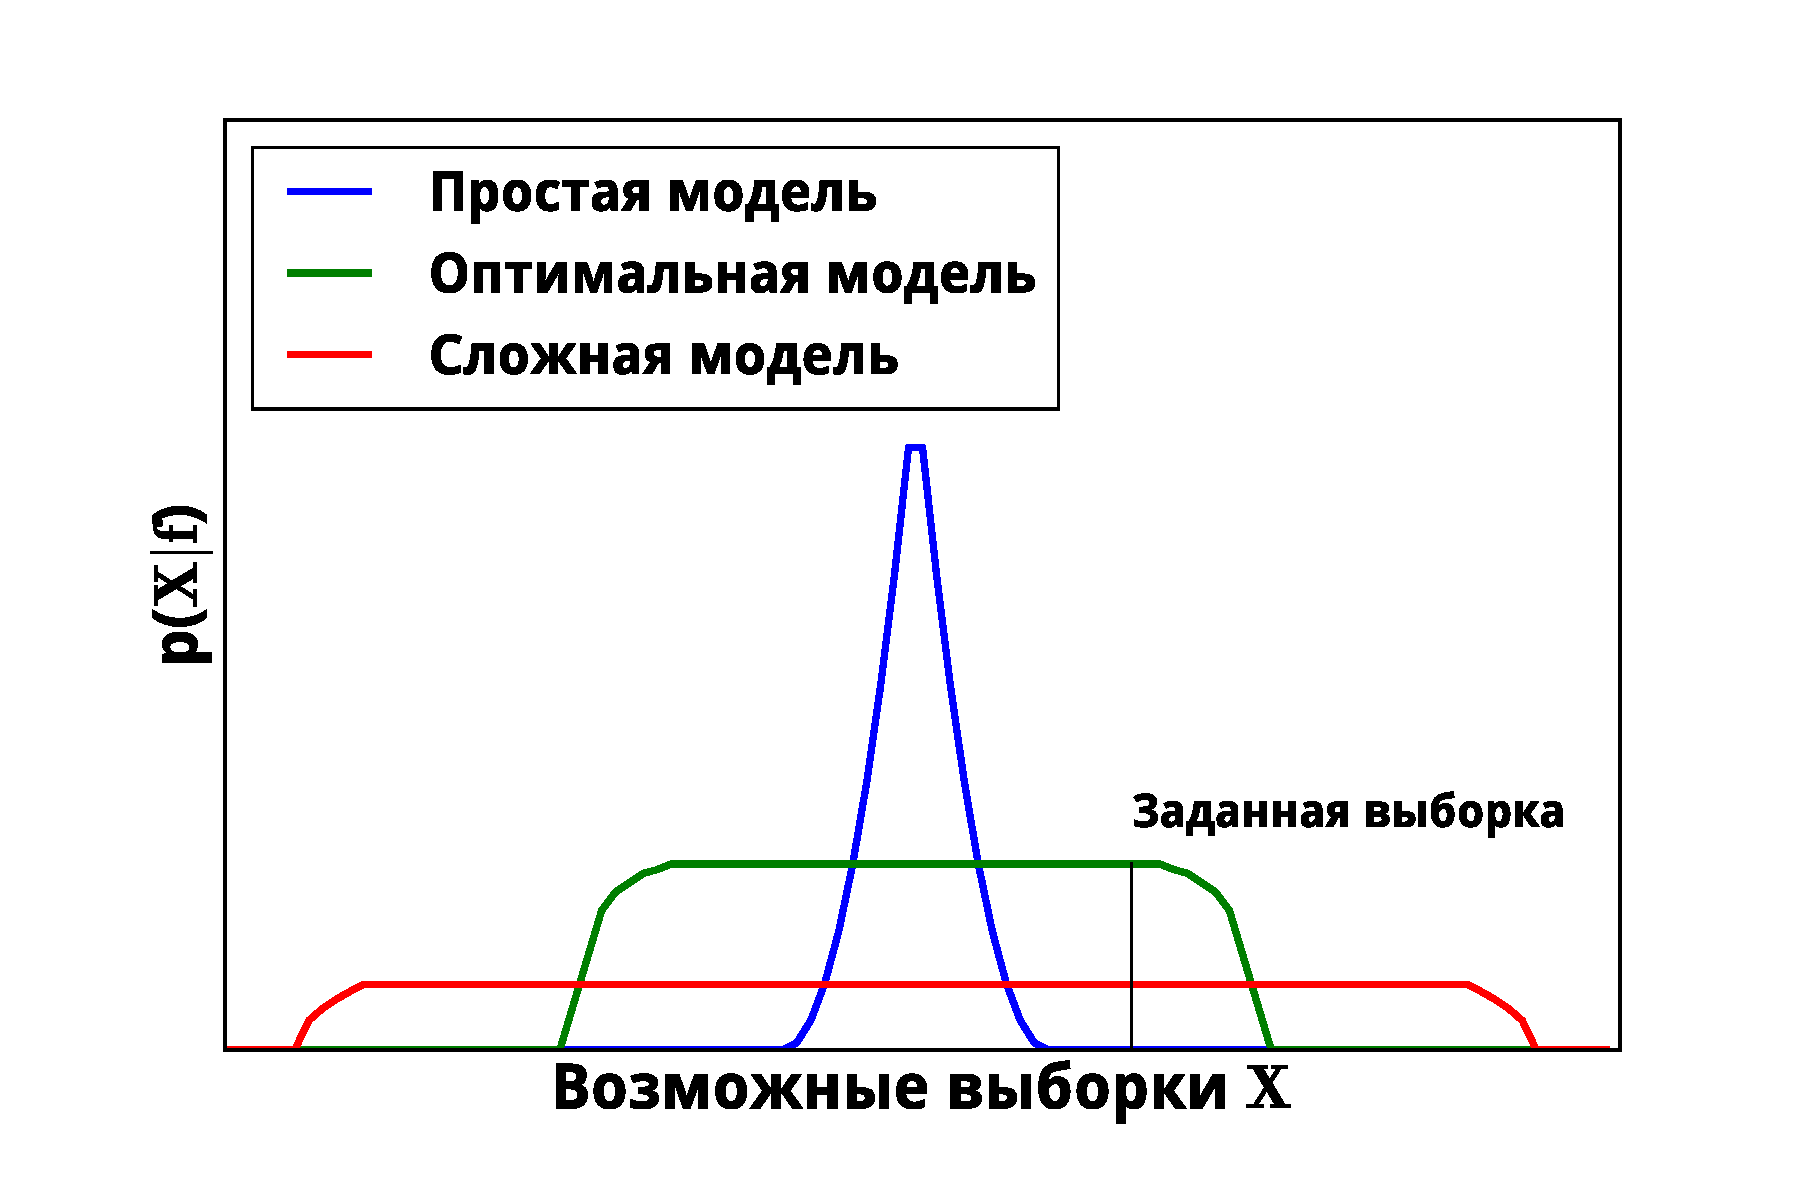
\includegraphics[width=0.4\textwidth]{evidence.pdf}} 
 \subfloat[Пример: полиномы]{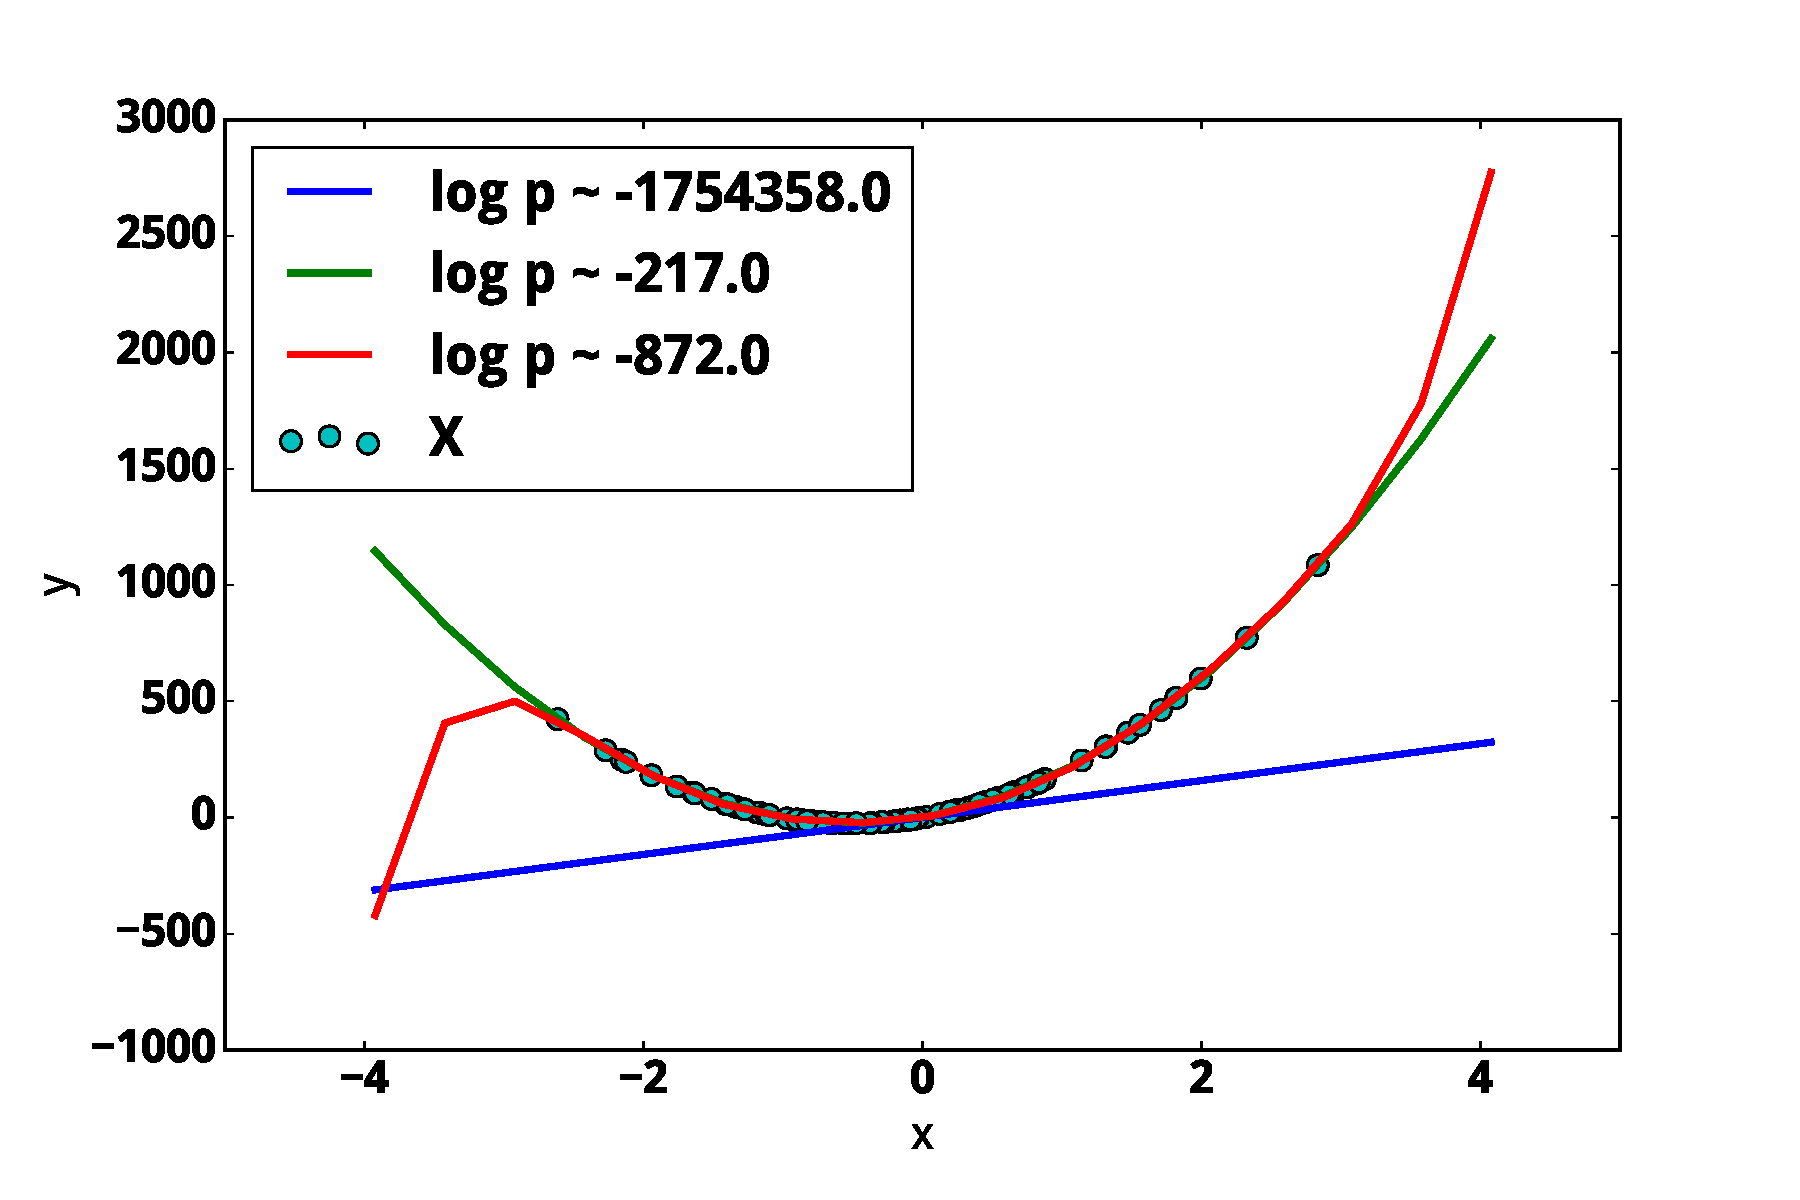
\includegraphics[width=0.4\textwidth]{example.pdf}}
\label{fig:1}\qquad

\end{figure}


\end{frame}

\begin{frame}{Байесовый подход к сложности}
Порождение vs описание\\
связь с Optimal MDL\\
Подбор априорных распределений
\end{frame}

\begin{frame}{Кросс-валидация vs Evidence}
Оценка Evidece:
\[
log~p(\mathbf{X}|\mathbf{f}) = log~p(\mathbf{x}_1|\mathbf{f}) + log~p(\mathbf{x}_2|\mathbf{x}_1, \mathbf{f}) + \dots +  log~p(\mathbf{x}_n|\mathbf{x}_1,\dots,\mathbf{x}_{n-1}, \mathbf{f}).
\]

Оценка leave-one-out:
\[
LOU = \mathsf{E} log~p(\mathbf{x}_n|\mathbf{x}_1,\dots,\mathbf{x}_{n-1}, \mathbf{f}).
\]

Кросс-валидация оценивает сложность описания одной части выборки при условии другой части выборки. \\
Evidence оценивает \textbf{полную} сложность описания заданной выборки.
\end{frame}

\begin{frame}{Методы получения оценок Evidence}
MC, Laplace
\end{frame}

\section{Вариационная нижняя оценка}
\begin{frame}{Вариационная оценка}
Зачем нужна, что такое
\end{frame}

\begin{frame}{Пример: логистическая функция}
Копипсата работы Адуенко
\end{frame}

\begin{frame}{Получение вариацонной оценки}
Формула получения нижней оценки
\end{frame}

\begin{frame}{$D_\text{KL}$}

\end{frame}

\begin{frame}{Пример: нормальное распределение}
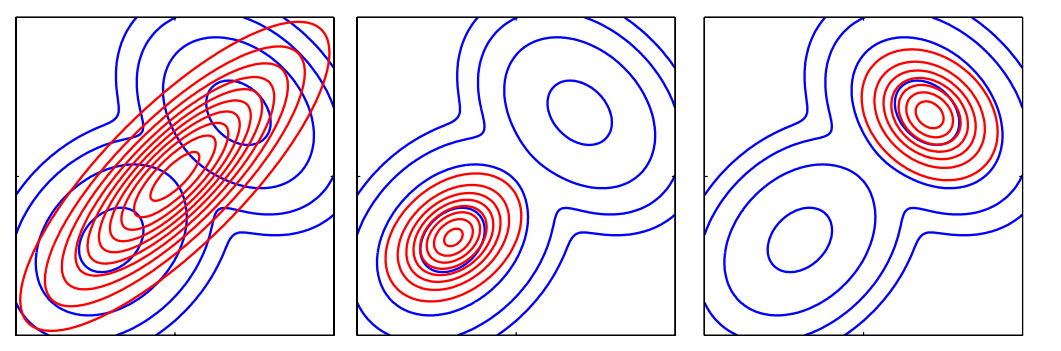
\includegraphics[width=\textwidth]{bishop.png}
\end{frame}


\begin{frame}{Использование вариационной нижней оценки}
\textbf{Для чего используют variational inference?}
\begin{itemize}
\item получение оценок Evidence;
\item получение оценок распределений моделей со скрытыми переменными (тематическое моделирование, снижение размерности).
\end{itemize}

\textbf{Зачем используют variational inference?}
\begin{itemize}
\item сводит задачу нахождения апостериорной вероятности к методам оптимизации;
\item проще масштабируется, чем аппроксимация Лапласа;
\item проще в использовании, чем MCMC.
\end{itemize}
\end{frame}


\section{Получение оценок для порождающих моделей}
\begin{frame}{Пример: автокодировщик}
Автокодировщик --- модель снижения размерности:
$$
	\mathbf{H} = \boldsymbol{\sigma}(\mathbf{W}_e \mathbf{X}),
$$
$$
	||\boldsymbol{\sigma}(\mathbf{W}_d\mathbf{H}) - \mathbf{X}||_2^2 \to \min.
$$

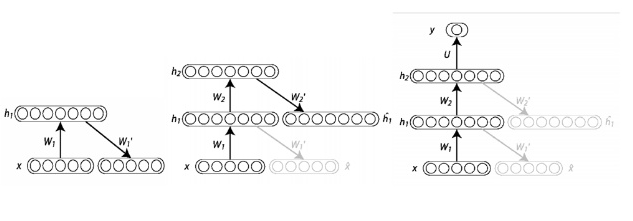
\includegraphics[width=\textwidth]{bengio.png}
\end{frame}



\begin{frame}{Автокодировщик как energy-based модель}
Интегралы и картинки из Bengio
\end{frame}

\begin{frame}{Вариационный автокодировщик}
Формулы
\end{frame}

\begin{frame}{Вариационный автокодировщик: правдоподобии модели}
Полная формула 
\end{frame}

\begin{frame}{Вариационный автокодировщик: правдоподобии модели}
Графики, примеры работы
\end{frame}

\section{Получение оценок для разделяющих моделей}
\begin{frame}{Разделяющие модели: правдоподобие}
аппроксимация нормальным распределением
\end{frame}

\begin{frame}{Градиентный спуск для оценки правдоподобия}
Иллюстрация
\end{frame}

\begin{frame}{Переобучение}
Иллюстрация
\end{frame}

\begin{frame}{Динамика Ланжевина}
иллюстрация
\end{frame}

\begin{frame}{Результаты}
\end{frame}

\end{document}

